\chapter{Optical potentials}

In the introduction we presented the concept of our envisaged potential
creation. In the following chapter we want to recapitulate the theoretical
foundations of optical lattice potentials and how it alters under an
additional optical potential well.

\section{Atom-light interaction}

At first we need to ask ourselves how the laser field propagates as
perturbation potential to the Hamiltonian of the atomic system and how we can
express said potential in terms of the intensity distribution we can control
throughout the experiment.

\subsection{Dipole potential}

We will use \gls{si} units if not noted else. The Hamiltonian of an electron
in an external electromagnetic field reads
\begin{equation}
  \hat{H}_\text{em}
  =\frac{1}{2m}\left(\hat{\vb{p}}+e\vb{A}\right)^2-e\Phi+\hat{V}_0
  \label{eq:hamiltonian_em}
\end{equation}
with vector potential $\vb{A}$ and scalar potential $\Phi$ of the external
field and the Coulomb potential of the nucleus $\hat{V}_0$.
\Cref{eq:hamiltonian_em} is exact for the hydrogen atom that only hosts one
electron. For alkali atoms we know that inner electron shells are closed and
the single outer electron is approximately described by
\cref{eq:hamiltonian_em}. The electromagnetic field relates to the
vector and scalar potential through
\begin{align}
  \vb{E}=-\grad{\Phi}-\pdv{\vb{A}}{t} &&
  \vb{B}=\curl{\vb{A}}
  \label{eq:field_em_potentials}
\end{align}
where $\vb{E}$ is the electric and $\vb{B}$ the magnetic field component.

\subsubsection{Gauge freedom}

Gauge freedom of the electromagnetic vector and scalar potential permit
transformations of kind
\begin{align}
  \vb{A}\to\vb{A}+\grad{\chi}
  &&
  \Phi\to\Phi-\pdv{\chi}{t}
  \label{eq:gauge_transform_em}
\end{align}
with gauge function $\chi(\vb{x},t)$.

We can see that insertion of \cref{eq:gauge_transform_em} into
\cref{eq:field_em_potentials} and applying vector calculus identities yields
expressions for the electromagnetic field components independent of the gauge
function $\chi$. We usually only consider the electromagnetic field to
represent physical reality, thus Gauge freedom describes physical redunancy
in mathematically distinct solutions.\footnote{The Aharonov-Bohm effect
actually provides evidence that also the electromagnetic potentials represent
physical reality.}

\subsubsection{Dipole approximation}

In the following we choose the gauge function $\chi=-\vb{A}\cdot\vb{x}$ and
assume the dipole approximation $\vb{A}(\vb{x},t)\approx\vb{A}(t)$. The
dipole approximation is reasonable as wave length of visible light are much
larger then atomic length scales \cite{Gerry2004}. In the dipole
approximation $\chi$ satisfies the Coulomb gauge condition
$\divergence{\vb{A}}=0$ allowing us to set $\Phi=0$ as no external sources
are present \cite{Jackson2005}. Finally we can rewrite
\cref{eq:hamiltonian_em} as
\begin{equation}
  \hat{H}_\text{dip}
  =\frac{\hat{\vb{p}}^2}{2m}+\hat{V}_0+\hat{V}_\text{dip}
  =\hat{H}_0+\hat{V}_\text{dip}
  \label{eq:hamiltonian_dip}
\end{equation}
with the dipole potential
\begin{equation}
  \hat{V}_\text{dip}
  =-\hat{\vb{d}}\cdot\vb{E}
  \label{eq:potential_dip},
\end{equation}
dipole operator $\hat{\vb{d}}=-e\vb{x}$ and spatially homogeneous light
field $\vb{E}(t)$.

\subsection{Effective potential}

We are now going to solve \cref{eq:hamiltonian_dip} for an arbitrary light
field of the form
\begin{equation}
  \vb{E}(t,\vb{x})
  =\vb{E}_0(\vb{x})\cos(\omega t)
  \label{eq:light_field}
\end{equation}
where $\vb{E}_0(\vb{x})$ should be compatible with Maxwell's equations and
be approximately constant on atomic length scales to not infringe with the
dipole approximation. Further we need the laser frequency $\omega$ to be
far-off-resonant to the atomic transition frequencies.

\subsubsection{General case}

At $t<0$ the system is in the energy eigenstate $\ket{n}$ of the
unperturbated Hamiltonian $\hat{H}_0$
\begin{equation}
  \hat{H}_0\ket{n}
  =E_n\ket{n}
  =\hbar\omega_n\ket{n}
  \label{eq:eigenvalue_energy_unperturbated}.
\end{equation}
At $t>0$ the external light field appears instantaneous. The new state
$\ket{\psi}$ can be expanded in the complete base of the previous energy
eigenstates
\begin{equation}
  \ket{\psi}
  =\sum_nc_n(t)e^{-i\omega_nt}\ket{n}
  \label{eq:state_expansion_unperturbated}.
\end{equation}
Inserting \cref{eq:state_expansion_unperturbated} into the time-dependent
Schrödinger equation with dipole Hamiltonian \cref{eq:hamiltonian_dip} and
applying $\bra{m}e^{i\omega_mt}$ to the right hand side leads us to a set
of differential equations
\begin{equation}
  \dot{c}_m
  =-\frac{i}{\hbar}\sum_nc_n(t)e^{-i\omega_{nm}t}\bra{m}\hat{V}_\text{dip}\ket{n}
  \label{eq:differential_equation_population_dynamics}
\end{equation}
with $\omega_{nm}=\omega_n-\omega_m$. The dynamics of the perturbated system
are described by the time-dependent probablity amplitudes $c_n(t)$.
By using \cref{eq:light_field} we can rewrite the dipole transition matrix
elements
\begin{equation}
  \bra{m}\hat{V}_\text{dip}\ket{n}
  =\Omega_{nm}(\vb{x})\cos(\omega t)\hbar
  \label{eq:elements_dipole_transition_matrix}
\end{equation}
where we introduced the Rabi frequency
\begin{equation}
  \Omega_{nm}(\vb{x})
  =\bra{n}\hat{\vb{d}}\cdot\vb{E}_0(\vb{x})\ket{m}/\hbar
  \label{eq:rabi_frequency}.
\end{equation}
Explicit values for general dipole transition elements for one and two
electron systems can be found in \cite{Bethe1957}. Transition elements
vanishes for states with same parity, in particular $\Omega_{nn}=0$
\cite{Bartelmann2018}.

\subsubsection{Two state system}

From now on we assume a two state system that initially is only populated in
the ground state $c_g(0)=1,c_e(0)=0$. Under these circumstances the dynamics
described in \cref{eq:differential_equation_population_dynamics} simplify to
\begin{align}
  i\dot{c}_g=\Omega_0c_e(t)\cos(\omega t)e^{+i\omega_0 t} &&
  i\dot{c}_e=\Omega_0c_g(t)\cos(\omega t)e^{-i\omega_0 t}
  \label{eq:differential_equation_population_dynamics_two_state_system}
\end{align}
with $\Omega_0=\Omega_{ge}(\vb{x})$. Expansion of $\cos(\omega t)$ in terms
of the exponential function and dropping $e^{\pm i(\omega+\omega_0)t}$ yields
\begin{align}
  i\dot{c}_g\approx\frac{\Omega_0}{2}c_e(t)e^{+i\Delta\omega t} &&
  i\dot{c}_e\approx\frac{\Omega_0}{2}c_g(t)e^{-i\Delta\omega t}
  \label{eq:differential_equation_population_dynamics_two_state_system_rwa}.
\end{align}
The so-called rotating wave approximation is motivated by the fact that
oscillations of frequency $\omega+\omega_0$ are fast compared to changes in
the population dynamics and therefore vanish on average.

We now define $a_g=c_g$ and $a_e=c_ee^{i\Delta\omega t}$ and refine
\cref{eq:differential_equation_population_dynamics_two_state_system_rwa} by
\begin{align}
  i\dot{a}_g=\frac{\Omega_0}{2}a_e(t) &&
  i\dot{a}_e=\frac{\Omega_0}{2}a_g(t)-a_e\Delta\omega
  \label{eq:differential_equation_population_dynamics_two_state_system_shift}.
\end{align}
In the former form we can diagonalize the Hamiltonian and find energy
eigenvalues to be
\begin{equation}
  E_{e,g}
  =\frac{\hbar}{2}\left(-\Delta\omega\mp\sqrt{\Omega_0^2+\Delta\omega^2}\right)
  \approx
  \mp\frac{\hbar\Omega_0^2}{4\Delta\omega}
  \label{eq:eigenvalues_energy_light_shift}
\end{equation}
where we applied Taylor expansion to the square root for
$\Delta\omega\gg\Omega_0$.

\subsubsection{AC light shift}

In result atoms in an external off-resonant light field experience an
effective periodic dipole potential
\begin{equation}
  \hat{V}_\text{eff}(\vb{x})
  =
  \mp\frac{\hbar\Omega_0^2(\vb{x})}{4\Delta\omega}
  =
  \mp\frac{d_0^2E_0^2(\vb{x})}{4\hbar\Delta\omega}
  \label{eq:potential_effective}
\end{equation}
with dipole element $d_0$. Same results can also be obtained by the use of
second order perturbation theory, however the presented approach is more
clear on assumptions and time dependence \cite{Grimm2008}.

\section{Laser light fields}

In this section our focus will be on the laser light field that creates the
optical lattice potential and the laser light field that creates the
time-averaged dynamic potentials.

\subsection{Gaussian beams}

The predominant output mode of most lasers is the fundamental transverse
gaussian mode described by
\begin{equation}
  \vb{E}(r,z)
  =
  \vb{E}_0\frac{w(0)}{w(z)}
  \exp{-\frac{r^2}{w(z)^2}}
  \exp{-ik\left(z+\frac{r^2}{2R(z)}-\arctan(\frac{z}{z_R})\right)}
  \label{eq:gaussian_beam}
\end{equation}
where $w(z)$ is the waist radius, $z_R=\pi w(0)^2/\lambda$ the Rayleigh
range and $R(z)$ the radius of curvature of the beam's wavefronts at $z$.

\begin{figure}[ht]
  \centering
  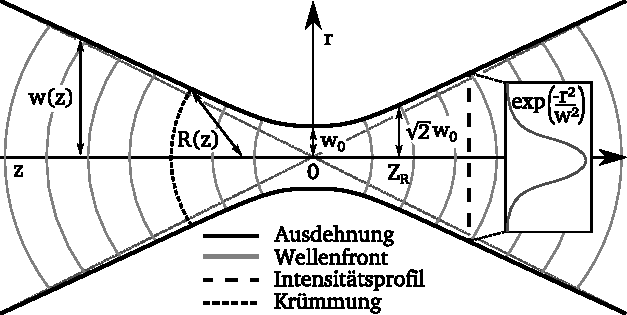
\includegraphics[width=.9\textwidth]{\mediadir{image/gaussian-beam.pdf}}
  \captionsetup{width=.9\textwidth}
  \caption{Illustration of gaussian beam parameters from $\aleph$ (Aleph),
    http://commons.wikimedia.org. The waist radius $w(z)$ relates to the beam
    width, $R(z)$ relates to the wavefront curvature and $z_R$ is the
    distance from origin $z=0$ where the beam width is $w(z)=\sqrt{2}w(0)$.}
  \label{fig:gaussian_beam}
\end{figure}

\Cref{fig:gaussian_beam} unveils how the parameters relate to the beam
profile propagation. The waist radius $w(z)$ corresponds to the beam width,
$R(z)$ relates to the wavefront curvature and $z_R$ is the distance from
origin $z=0$ where the beam width is $w(z)=\sqrt{2}w(0)$. Beam width
and curvature radius evolve according to
\begin{align}
  w(z)=w(0)\left[1+\left(\frac{z}{z_R}\right)^2\right]^{1/2}
  &&
  R(z)=z\left[1+\left(\frac{z_R}{z}\right)^2\right]
  \label{eq:gaussian_beam_evolvement}.
\end{align}

Fortunately \cref{eq:potential_effective} only depends on the absolute
square of the electric field, thus we can drop the complex exponential from
\cref{eq:gaussian_beam} to find an expression for the Gaussian intensity
distribution
\begin{equation}
  I(r,z)
  =
  I_0
  \left(\frac{w(0)}{w(z)}\right)^2
  \exp{-\frac{2r^2}{w(z)^2}}
  =
  I_0
  \frac{\exp{-\frac{2r^2}{w(z)^2}}}{1+\left(\frac{z}{z_R}\right)^2}
  \label{eq:gaussian_intensity}
\end{equation}
where $I_0$ is the maximum intensity at $r=z=0$.

\subsubsection{Lattice intensity}

An one dimensional optical lattices can be generated through the interference
of two counter-propagating Gaussian beams
\begin{align*}
  \vb{E}_\rightarrow(\vb{x},t)+\vb{E}_\leftarrow(\vb{x},t)
  &=
  \vb{E}_0(r,z)\cos(kz-\omega t)+\vb{E}_0(r,z)\cos(kz-\omega t)\\
  &=
  2\vb{E}_0(r,z)\cos(kz)\cos(\omega t)
\end{align*}
Therewith the intensity distribution equals
\cref{eq:gaussian_intensity} with an additional $4\cos^2(kz)$ factor
\begin{equation}
  I(z)
  =
  4I_0\cos^2(kz)
  \frac{\exp{-\frac{2r^2}{w(z)^2}}}{1+\left(\frac{z}{z_R}\right)^2}
  \label{eq:lattice_intensity}
\end{equation}
contributed through the constructive interference.

\begin{table}[h]
  \centering
  \begin{tabular}{|c|c|c|c|}
    \hline
    Laser wavelength $\lambda$ &
    Lattice constant $a=\lambda/2$ &
    Beam waist $w(0)$ &
    Rayleigh length $z_R$ \\
    \hline
    \SI{1064}{\nano\meter} &
    \SI{532}{\nano\meter} &
    \SI{150}{\micro\meter} &
    \SI{66}{\milli\meter} \\
    \hline
  \end{tabular}
  \captionsetup{width=.8\textwidth}
  \caption{Typical values for a Gaussian beam used to construct an optical
    lattice potential.}
  \label{tab:gaussian_beam_lattice}
\end{table}

\Cref{tab:gaussian_beam_lattice} lists typical values for a Gaussian beam
used to construct an optical lattice potential. Optical lattices have up to
50 lattice sites spanning over a range of $l=50a\approx\SI{27}{\micro\meter}$
\cite{Rom2009}. For $-l/2<z<+l/2$ we find that $w(z)\approx w(0)$ and because
$r\ll1$ we can approximate \cref{eq:lattice_intensity} to follow
\begin{equation}
  I(z)
  \approx
  4I_0\cos^2(kz)
  \label{eq:gaussian_intensity_approx}
\end{equation}
which we will use from now on as the intenisty distribution for one
dimensional optical lattices.

\subsubsection{Perturbation intensity}

The laser beam used to perturbate the optical lattice potential has slightly
different parameters \cite{Hertlein2017} as we can see in
\Cref{tab:gaussian_beam_perturbation}.

\begin{table}[h]
  \centering
  \begin{tabular}{|c|c|c|c|}
    \hline
    Laser wavelength $\lambda$ &
    Beam waist $w(0)$ &
    Rayleigh length $z_R$ \\
    \hline
    \SI{532}{\nano\meter} &
    \SI{1}{\micro\meter} &
    \SI{6}{\micro\meter} \\
    \hline
  \end{tabular}
  \captionsetup{width=.8\textwidth}
  \caption{Typical values for a Gaussian beam used to perturbate the optical
    lattice potential reported by \cite{Hertlein2017}.}
  \label{tab:gaussian_beam_perturbation}
\end{table}

For these parameters approximations made for optical lattice are not valid
and we need to the exact \cref{eq:gaussian_intensity} formula.

\section{Potential interaction}

We have now found two different expressions for the intensity of the optical
lattice and of the perturbation. We will now further assume
$V_{\text{lat}}(0)=-10E_r$ and $V_{\text{per}}(0)=+2E_r$. In addition we
expect the perturbation to be directed at six different points. Under these
circumstances we expect the effective potential, the superposition from the
lattice potential and the perturbation to evolve as depicted in
\Cref{fig:perturbated_potential_evolution}.

\begin{figure}[ht]
  \centering
  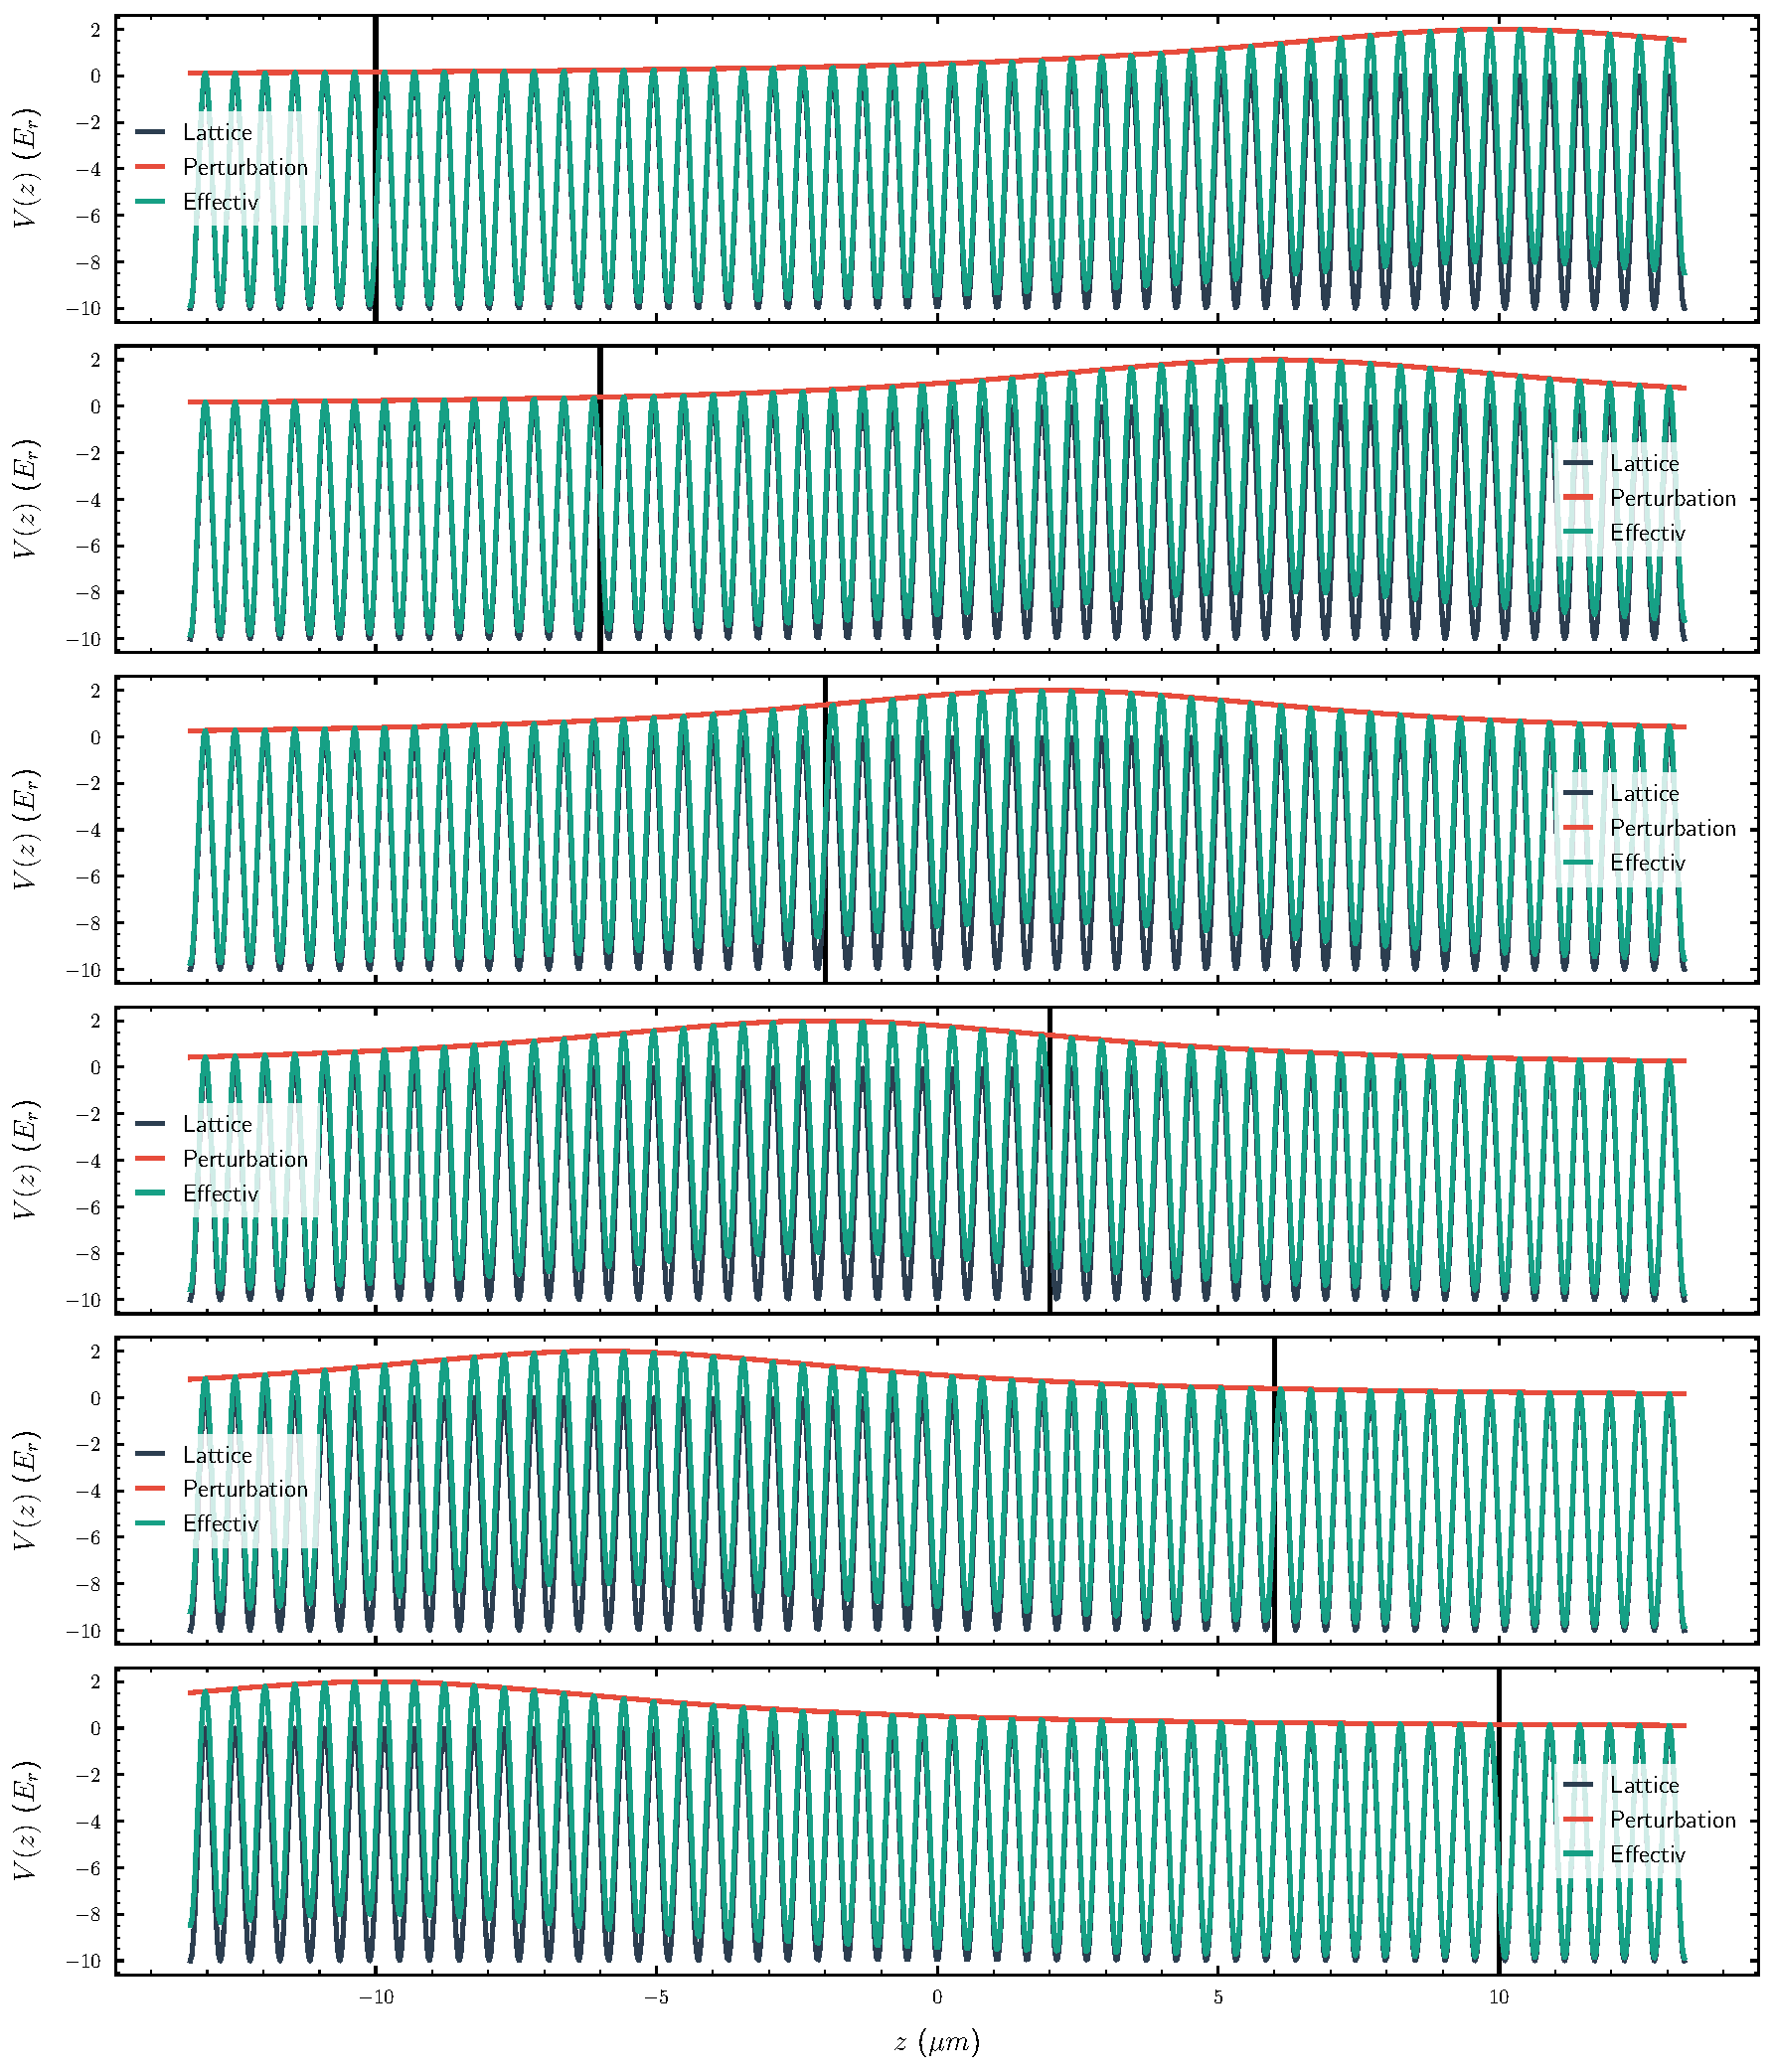
\includegraphics[width=\textwidth]{\figuredir{potential/evolution.pdf}}
  \captionsetup{width=.9\textwidth}
  \caption{Time evolution of local perturbated potentials. We can see how
    the perturbated potential changes within the spatial coordinates (black
    vertical line) in comparison to the periodic lattice potential.}
  \label{fig:perturbated_potential_evolution}
\end{figure}

We can clearly see how the different beam parameters affect the intensity
distribution and thereby the potential shape. Further we see how the
perturbation wanders (black vertical line) accross the spatial dimension.

\begin{figure}[ht]
  \centering
  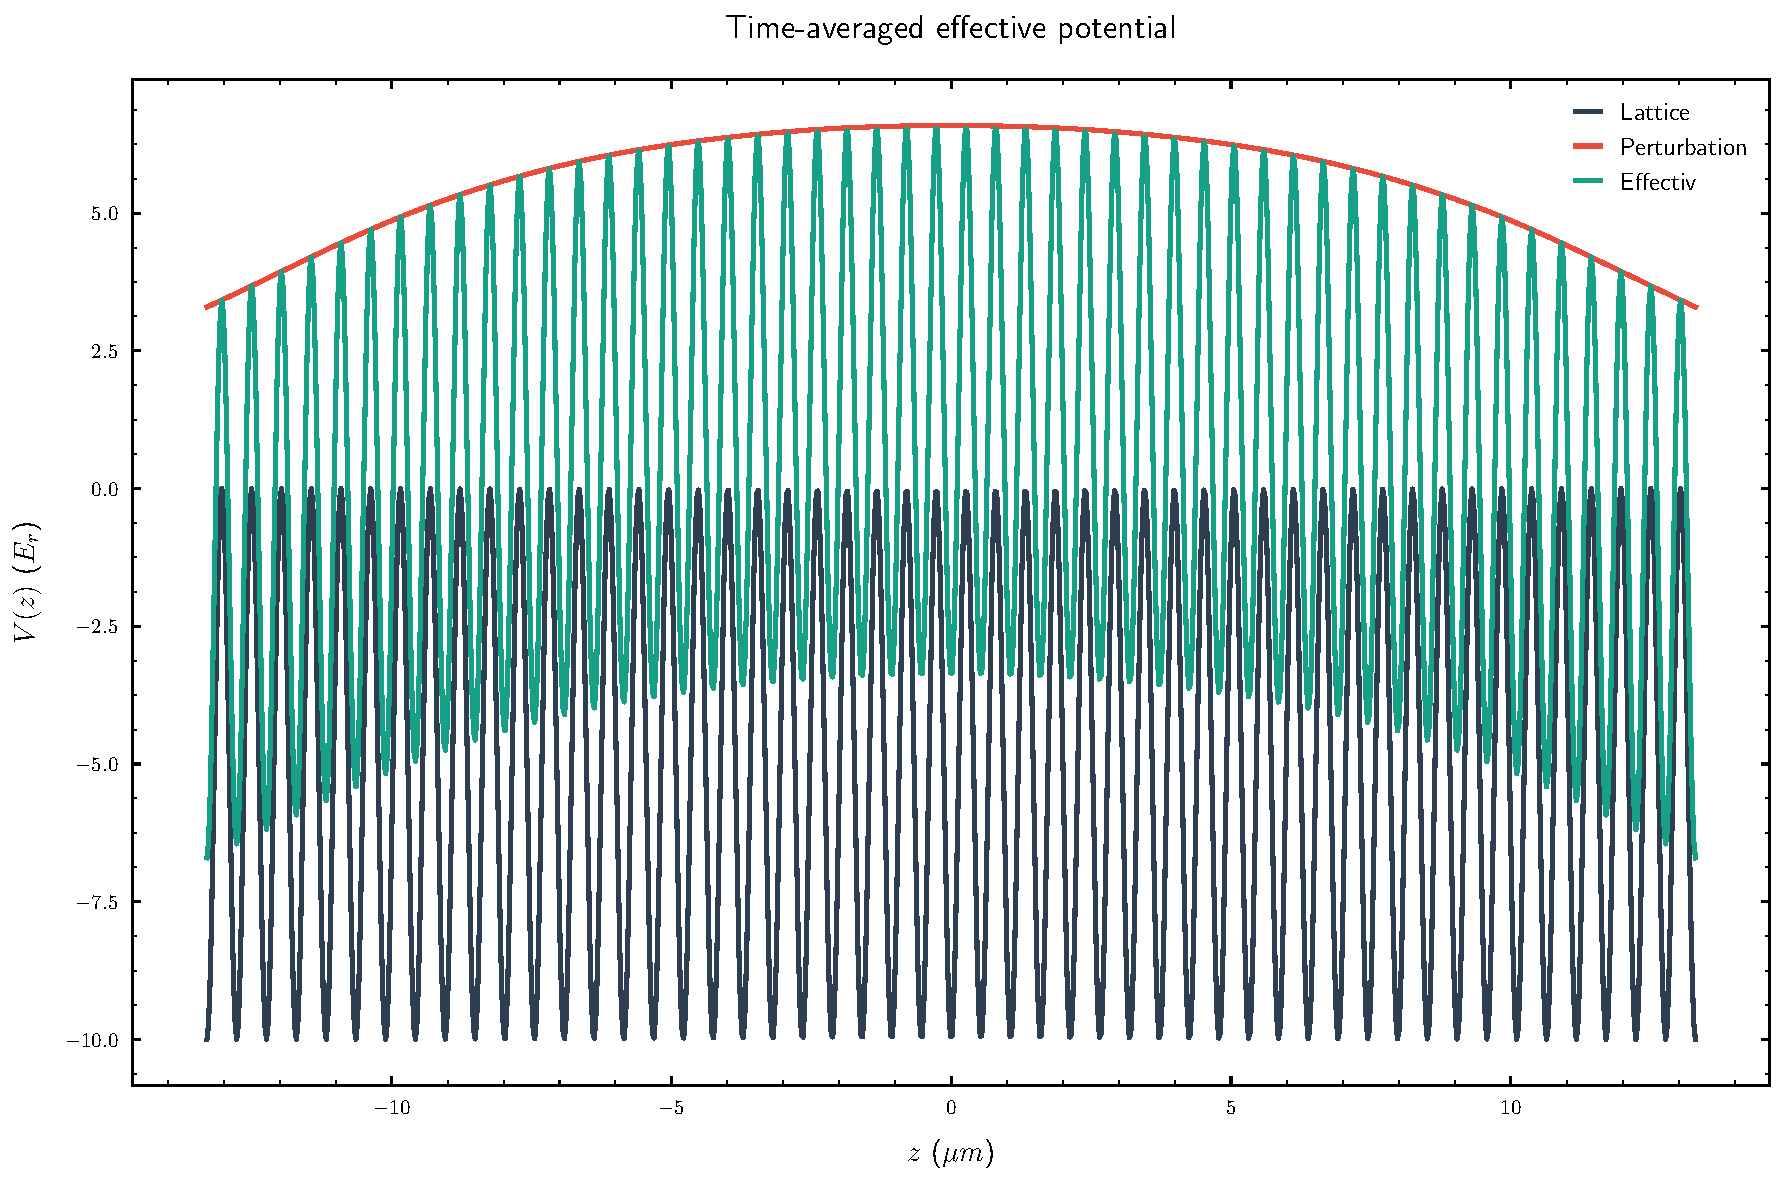
\includegraphics[width=\textwidth]{\figuredir{potential/effective.pdf}}
  \captionsetup{width=.9\textwidth}
  \caption{Time average of local perturbated potentials. Over a time average
  we see that the perturbation causes a local potential shift on top of the
lattice potential.}
  \label{fig:perturbated_potential_effective}
\end{figure}

In \Cref{fig:perturbated_potential_effective} we created the time-average
from the perturbation states. We can see how the time-average yields an
approximate localized potential energy shift.

